% =============================================================================
% CS7980 Capstone paper — WEEK-13 REVISION (作业版).
% Base: Sharon's capstone_week11_full.tex (feat/e3-rap-portal-industrial,
% c301c7f) — kept verbatim wherever possible. This revision folds in the
% decorrelation/tooling content (docs 14, 16-19) that the superseded
% capstone_week12_full.tex carried, reworded per Sharon's 10-point review:
%   #1 subtitle "...of Decorrelation and Its Limits" + early bridge paragraph;
%   #3 no "only variable" overclaims (week11 adjacent-contrasts wording kept);
%   #5 uses the week11 4-panel figure;
%   #6 module matched-budget control reported as n.s. (no unsourced p-value);
%   #7 "agentless-ungrounded" -> defined inline as single-pass diff-only;
%   #8 RQ3 answered (week11 Section IV-G kept);
%   #9 "survives a change of pair judge" wording (no "judge-invariant");
%   #10 "eleven sources" (not models) + Nova union/judge circularity disclosed.
% New sections: IV-E ladder+ceiling+linter, IV-F capability/structure nulls,
% IV-G execution probe. New refs: crab, swereview.
% PR #41 evidence upgrades ported verbatim (all four hunks): run-stability
% sentence (III-A), paired rank-biserial agreement (III-C), TOST equivalence +
% MDE (IV-A), Gwet AC1/PABAK kappa-paradox robustness (completeness).
%
% Remaining TODO (homework scope; OSF DOI not needed for a class submission):
%  - Fig. 1's embedded title duplicates the LaTeX \caption and reads
%    "...Topologies" while the paper now says "Workflows". Crop the top title
%    banner from fig1_architectures_week11.png (or relabel "Topologies" ->
%    "Workflows"). The three earlier image-content fixes (rung-capability
%    banner, "Deterministic" labels, dropping "Same Roles") are already done in
%    this version of the figure.
% =============================================================================

\documentclass[conference]{IEEEtran}
\IEEEoverridecommandlockouts

\usepackage{cite}
\usepackage{amsmath,amssymb,amsfonts}
\usepackage{graphicx}
\usepackage{booktabs}
\usepackage{textcomp}
\usepackage{xcolor}
\usepackage{url}

\begin{document}

\title{Evaluating Decorrelation in LLM Code Review:\\
A Pre-Registered Study}

\author{\IEEEauthorblockN{En-Ping Su, Tong Wu, Shiting Huang, Mengshan Li}
\IEEEauthorblockA{\textit{Khoury College of Computer Sciences} \\
\textit{Northeastern University}, Vancouver, Canada}}

\maketitle

\begin{abstract}
Large Language Models are increasingly used for automated code review, and
multi-agent frameworks propose dividing the work among specialized agents. It
remains unclear whether the \emph{structure} of that collaboration---rather than
the agents' mere presence, or the extra compute they consume---improves review
quality; only reviews whose errors are \emph{decorrelated} can be combined into a
better one. Under a pre-registered, compute-matched design, we compare a
four-rung experimental \emph{ladder} that incrementally adds sampling, role
specialization, and peer communication---an Agentless single-LLM baseline, a
compute-matched Generalists-3 control, a Hierarchical manager-plus-specialists
design, and a Decentralized Peer Consensus design---holding the model, PR
snapshot, prompts, and evaluation pipeline fixed, across three datasets:
injected-defect ground truth, human-reviewed PRs, and a live industrial
repository. Three findings emerge. \emph{Communication is not the lever:} role
specialization yields no improvement over compute-matched sampling ($p{=}0.73$),
and no multi-agent workflow exceeds the single-pass baseline's F1, buying recall
only at 3--9$\times$ the call budget. \emph{Verification is:} findings that
independent model families agree on match injected ground truth 89\% of the time
versus 54\% for one model repeating itself---error decorrelation paying on
precision, not coverage. \emph{Grounding bounds both:} unioning every
configuration we ran plateaus at a ${\approx}0.83$ recall ceiling whose residue
is mechanical conventions a linter recovers and a functional hard-core that
execution, not more reading, begins to reach; and on unlabeled industrial code
the verification relationship reaches its ecological boundary, because LLM
correctness judges themselves disagree ($\kappa{=}0.03$).
\end{abstract}

\begin{IEEEkeywords}
Large Language Models, Multi-Agent Systems, Automated Code Review, Evaluation,
LLM-as-a-Judge.
\end{IEEEkeywords}

% =============================================================================
\section{Introduction}

Code review gates most software changes, and LLMs now plausibly automate parts
of it. A prominent design direction decomposes the task among specialized agents
that communicate, as in ChatDev~\cite{chatdev} and MetaGPT~\cite{metagpt}. Most
evaluations, however, compare a \emph{whole} multi-agent system against a single
model, conflating additional computation with workflow structure---how many
agents there are versus how they are organized. We ask:

\begin{quote}
\textbf{RQ:} Holding the underlying model, review target, and evaluation
procedure fixed, what incremental effects do additional sampling, role
specialization, and inter-agent communication have on the effectiveness and
efficiency of automated code review?
\end{quote}

Answering this needs a control most studies omit: if a three-specialist team
beats a single reviewer, the cause may be three samples rather than three
\emph{roles}. We therefore add a compute-matched \textbf{Generalists-3}
arm---the same prompt sampled three times and merged---so specialization is
tested against equal compute (Agentless remains a strong single-pass
baseline~\cite{agentless}). This exposes the paper's organizing idea,
\emph{error decorrelation}: additional reviewers improve quality only insofar as
their mistakes are independent, so the question throughout is whether a given
form of structure decorrelates a reviewer's errors or merely repeats them.

Because a benchmark result is only as trustworthy as its evaluation, we evaluate
on three complementary datasets---injected-defect ground truth, human-reviewer
agreement, and a live industrial repository---and pre-registered the hypotheses,
sample sizes, and analysis before collection. Our contributions are:
\begin{itemize}
  \item A pre-registered adjacent-contrast evaluation (2{,}415 reviews) isolating
  sampling, specialization, and communication.
  \item Evidence that homogeneous multi-agent workflows improve recall but not
  F1, while agreement between independent model families is a precision signal.
  \item Evidence that grounding---not additional communication---is the remaining
  bottleneck: a ${\approx}0.83$ recall ceiling whose residue is lint-targetable
  conventions and a repo-integrated functional core, bounded by an industrial
  case study where the verification signal cannot be validated without an oracle
  ($\kappa{=}0.03$).
\end{itemize}

\textbf{Scope and thread.} The registered study isolates the workflow axis and
its answer is largely null; the exploratory extensions
(Sections~\ref{sec:ceiling}--\ref{sec:execution}) trace \emph{why}, reducing
every movable lever to one axis---how \emph{decorrelated} the reviews are---which
pays on precision, not coverage. We mark confirmatory and exploratory claims
explicitly throughout.

% =============================================================================
\section{Related Work}

\textbf{LLM-based software engineering.} SWE-bench established that realistic
GitHub tasks are hard for language models~\cite{swebench}, and Agentless shows a
simple non-agent pipeline is competitive~\cite{agentless}---the natural baseline
for asking whether multi-agent communication adds value.

\textbf{Multi-agent software engineering.} ChatDev~\cite{chatdev} and
MetaGPT~\cite{metagpt} organize development as communication among role agents;
surveys find the area promising but under-evaluated~\cite{survey}, and recent
work catalogs \emph{why} such systems fail---coordination overhead, cascading
errors, weak verification~\cite{whyfail}. Concurrent 2026 results agree: agent
teams can hold experts back~\cite{pappu}, and mixing models does not beat the
best single model~\cite{selfmoa}.

\textbf{Verification and LLM judges.} LLM judges scale
evaluation~\cite{llmjudge}, verifier-based selection converts extra samples into
quality~\cite{cobbe}, and diverse judge panels can replace a single
judge~\cite{verga}, though judges show self-preference~\cite{panickssery} and
prompt-form sensitivity~\cite{sclar}.

Across this literature the assumption is that better coordination or
specialization yields better review, yet none isolates compute from communication
or tests error \emph{decorrelation} directly---which is what our compute-matched
adjacent-contrast design does, alongside a non-circular objective/subjective judge
split and a powered test of the correlated-error conjecture~\cite{zietsman}.

% =============================================================================
\section{Study Design}

\subsection{The four-rung ladder}
\label{sec:variables}
Each rung adds exactly one capability over its predecessor
(Fig.~\ref{fig:architectures}): (1)~\textbf{Agentless}---one LLM reviews the PR
in a single pass; (2)~\textbf{Generalists-3}---the same generalist prompt sampled
three times and merged, with no roles and no communication (the compute-matched
control that isolates sampling from specialization); (3)~\textbf{Hierarchical}---a
\emph{deterministic} coordinator routes the diff to frontend, backend, and
database specialists, whose findings a \emph{deterministic} synthesizer merges;
(4)~\textbf{Consensus}---the same specialists review independently, then exchange
findings and vote.

Hierarchical routing and synthesis are deterministic code, so its three LLM
calls are exactly its three specialists; only Consensus adds inference stages
(nine calls). The model (Claude Haiku 4.5, with a Sonnet 4.5 robustness arm in
Sections~\ref{sec:generation} and \ref{sec:nulls}), prompts, per-PR snapshot, and
evaluation pipeline are fixed; only sampling budget, roles, and message flow
vary, so we read \emph{adjacent} contrasts rather than treating topology as a
single isolated variable. Each (PR, arm) value is the mean of three runs; run
variance is negligible (within-PR SD of semantic F1 ${\approx}0.01$--$0.05$) and
the headline ordering holds in each run individually.

\begin{figure*}[t]
  \centering
  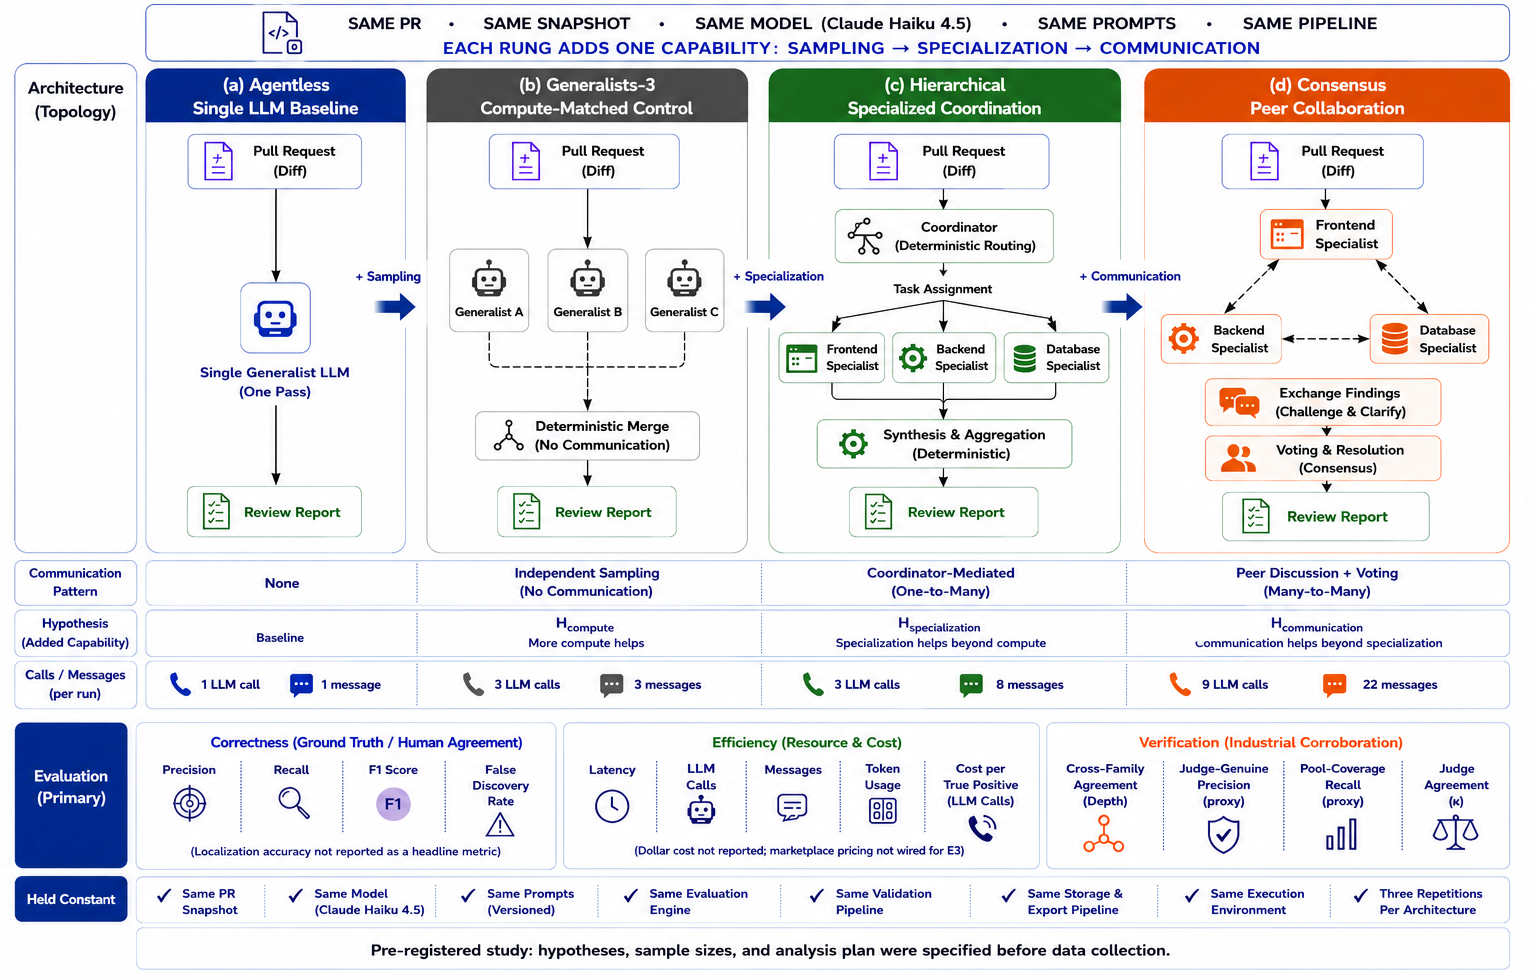
\includegraphics[width=\textwidth]{fig1_architectures_week13.png}
  \caption{The four-rung ladder. Adjacent contrasts add sampling, then
  specialization, then communication, while the PR snapshot, model, prompt
  templates, and evaluation pipeline are held constant and only the inference
  budget varies. Coordination and synthesis in the Hierarchical arm are
  \emph{deterministic}, so its three LLM calls are exactly its three specialists;
  Consensus adds peer discussion and voting (nine calls). Per-run call and
  message counts (below each rung) are the overhead in
  Table~\ref{tab:confirmatory}.}
  \label{fig:architectures}
\end{figure*}

\subsection{Datasets and metrics}
Table~\ref{tab:datasets} summarizes the three datasets. E3's 627 reviews are the
four-arm ladder plus single-pass cross-family arms (Haiku~4.5/Kimi~K2.5/GLM~5,
three runs each; GLM usable on 29/30 PRs).

\begin{table}[t]
\caption{Evaluation datasets.}
\label{tab:datasets}
\centering
\footnotesize
\begin{tabular}{@{}llll@{}}
\toprule
& PRs & Reviews & Correctness signal \\
\midrule
E1 Qodo         & 99 & 1{,}188 & injected ground truth (P/R/F1) \\
E2 SWE-PRBench  & 50 & 600     & human-reviewer agreement \\
E3 industrial   & 30 & 627     & corroboration proxies (no oracle) \\
\bottomrule
\end{tabular}
\end{table}

Findings are matched both strictly (file$+$line) and \emph{semantically} via an
independent LLM judge's binary same-issue decision (threshold-insensitive across
0.5--0.9); malformed findings are dropped and logged, not failed, removing a
survivorship bias against the single-call arm. Operational metrics (latency,
tokens, calls, messages) are collected identically. Lacking an oracle, E3
substitutes corroboration proxies on the cross-\emph{family} axis (the only one
that carries signal, Section~\ref{sec:hetero}): \emph{depth} clusters independent
findings with an LLM pair judge (Nova~Pro, $\tau{=}0.7$) and counts the model
families agreeing; \emph{proxy precision} is a separate judge's genuine-rate, and
\emph{proxy recall} is leave-one-out cross-family pool coverage.

\subsection{Hypotheses and analysis}
The design, hypotheses, sample sizes, and analysis plan were pre-registered on
OSF and prompts frozen before confirmatory collection. The registered contrasts
are summarized with their outcomes in Table~\ref{tab:hyp}. Two secondary
hypotheses were added by a pre-data amendment: \textbf{H-verify} (a
self-consistency filter lifts each multi-agent arm's F1 to within 0.02 of
Agentless) and \textbf{H-hetero-precision} (findings corroborated by ${\geq}2$ of
three independent families \{Haiku 4.5, Kimi K2.5, GLM~5\} gain ${\geq}10$
precision points at equal-or-higher F1, and all-three agreement exceeds the
frozen model's own three-run recurrence by ${\geq}10$ points). A further
pre-data amendment registered a capability contrast (Section~\ref{sec:nulls}).

The PR is the unit of analysis; contrasts use paired Wilcoxon signed-rank tests
with bootstrap CIs and Holm--Bonferroni correction within each hypothesis family,
and Cliff's $\delta$ as an unpaired magnitude. The registered paired $\delta$
differed from the implemented unpaired form; both indicate negligible effects
($r{=}{-}0.05$ vs.\ $\delta{=}{-}0.005$) and do not alter conclusions. All
statistics replay deterministically from persisted artifacts with zero new LLM
calls.

% =============================================================================
\section{Results}
\label{sec:results}

\begin{table}[t]
\caption{Registered hypotheses and confirmatory outcomes.}
\label{tab:hyp}
\centering
\footnotesize
\begin{tabular}{@{}p{1.55cm}p{2.6cm}p{3.0cm}@{}}
\toprule
\textbf{Hypothesis} & \textbf{Prediction} & \textbf{Outcome} \\
\midrule
H-specialization \emph{(primary)} & Specialists beat compute-matched generalists & \textbf{Null} ($p{=}0.73$) \\
H-compute        & 3 samples beat 1 & Supported on recall (0.63 vs.\ 0.50), not F1 \\
H-communication  & Consensus beats Hierarchical & Unsupported (Holm $p{=}0.12$) \\
H-efficiency     & Cost rises along the ladder & Supported (monotonic) \\
H-complexity     & Effect grows with PR complexity & Registered test unavailable; not supported under an exploratory proxy \\
H-verify         & Self-consistency restores parity & \textbf{Fails} \\
H-hetero-prec.\  & Cross-family agreement lifts precision & \textbf{Confirmed} (both sub-claims) \\
\bottomrule
\end{tabular}
\end{table}

\subsection{Generation axis: more agents buy recall, never quality}
\label{sec:generation}
Table~\ref{tab:confirmatory} gives per-arm means over the 99 Qodo PRs together
with the cost of obtaining them. The \textbf{primary hypothesis is null}: at
matched compute, Hierarchical ties Generalists-3 on recall (0.624 vs.\ 0.626;
$p{=}0.73$, $\delta{=}{-}0.005$) at comparable precision. The recall difference
is statistically \emph{equivalent} within the pre-registered $\pm6$-point SESOI
(TOST $p{<}0.001$; $90\%$ CI $[-0.025,0.019]$), so any specialization benefit is
below practical significance, not merely undetected---consistent with concurrent
evidence that teams average rather than exploit expertise~\cite{pappu}. Nor does compute
convert into quality: Agentless dominates every multi-agent arm on semantic F1
(0.487 vs.\ 0.357--0.378; all Holm $p{<}0.001$, $\delta$ 0.30--0.36). What extra
compute buys is recall---Generalists-3 and Hierarchical reach 0.62--0.63 vs.\
0.503 (Holm $p{<}0.001$)---though Consensus, the most expensive arm, does not
(0.536, Holm $p{=}0.12$): the full peer-consensus workflow did not outperform the
hierarchical one despite nine calls vs.\ three, leaving H-communication
unsupported. The trade is stark (Fig.~\ref{fig:support}a): one confirmed finding
costs 0.34 LLM calls under Agentless and 1.76 under Consensus, a $5\times$ premium
for a lower-F1 review; the operational ladder rises monotonically in messages,
latency, and cost-per-TP (H-efficiency).

On SWE-PRBench the shape replicates in natural data: Generalists-3 raises
coverage of human comments (0.68 vs.\ 0.51, Holm $p{=}0.001$; Hierarchical 0.63,
$p{=}0.05$), but F1 is a four-way tie (0.325 vs.\ 0.329--0.357, all n.s.,
$|\delta|{\le}0.06$). A registered Sonnet~4.5 robustness arm, now completed at
confirmatory scale ($N{=}99$), confirms the ordering is not a Haiku artifact:
every registered conclusion replicates---the specialization null (Hierarchical
vs.\ Generalists-3 recall median paired $\tilde\Delta{=}0.000$), Agentless F1
dominance (0.547 vs.\ 0.389--0.428, Holm $p{<}0.001$, $\delta$ 0.32--0.45), the
recall-not-F1 pattern, and H-verify's failure. Absolute F1 rises with the
stronger model (Agentless $0.487{\to}0.547$) but the ranking and every claim
are model-robust.

Finally, the pre-registered rescue fails. A self-consistency filter (keep
findings recurring in ${\geq}2$ of 3 runs) leaves Hierarchical at 0.378
($\tilde\Delta{=}{-}0.127$, CI $[-0.179,-0.083]$) and Consensus at 0.373
($\tilde\Delta{=}{-}0.114$), both entirely below the registered parity band;
$k{=}3$ fails for every arm. A model that agrees with itself is mostly repeating
its confident errors---which motivates the next section.

\begin{table}[t]
\caption{E1 (Qodo, 99 PRs): review quality and inference overhead. Agentless is
precision- and F1-dominant; extra agents buy recall at 3--9$\times$ the calls.
FDR $=1-$precision; Cost/TP $=$ LLM calls per confirmed true positive.}
\label{tab:confirmatory}
\centering
\footnotesize
\begin{tabular}{@{}lccccrrr@{}}
\toprule
\textbf{Arm} & \textbf{P} & \textbf{R} & \textbf{F1} & \textbf{FDR} & \textbf{Calls} & \textbf{Msgs} & \textbf{Cost/TP} \\
\midrule
Agentless      & \textbf{0.525} & 0.503 & \textbf{0.487} & \textbf{0.475} & 1 & 1  & \textbf{0.34} \\
Generalists-3  & 0.270 & \textbf{0.626} & 0.357 & 0.730 & 3 & 3  & 0.45 \\
Hierarchical   & 0.294 & 0.624 & 0.378 & 0.706 & 3 & 8  & 0.50 \\
Consensus      & 0.322 & 0.536 & 0.369 & 0.678 & 9 & 22 & 1.76 \\
\bottomrule
\end{tabular}
\end{table}

\subsection{Verification axis: cross-family agreement is a precision instrument}
\label{sec:hetero}
The registered companion generated agentless reviews with two independent
frontier families (Kimi K2.5, GLM~5), matched cross-model by a fourth family
(Nova Pro) as pair judge to keep the chain non-circular, and tested on the
registered 80-PR remainder. \textbf{Both sub-claims hold.} Findings corroborated
by ${\geq}2$ families reach per-PR precision 0.716 vs.\ 0.575 single-arm
($\bar\Delta{=}{+}0.141$, CI $[0.094,0.189]$, $p{<}10^{-4}$, $\delta{=}0.364$) at
equal-or-higher F1, and findings all three families produce are golden-matched
\textbf{89\%} of the time versus \textbf{54\%} for one model's three-run
recurrence (gap ${+}0.348$, CI $[0.286,0.412]$).

Fig.~\ref{fig:depth} makes the mechanism visible. Cross-family agreement climbs
steeply with depth; same-model recurrence stays flat before saturating at its
error ceiling. A second run of the same model contributes almost no independent
evidence; a second independent family does. The instrument survives a change of
pair judge---re-judging all 8{,}061 candidate pairs with a second pair judge
agrees at $\kappa{=}0.952$ and reproduces the rows.

\begin{figure}[t]
\centering
% Generated by figures/make_figures.py (or figures/figures.ipynb). Regenerate
% with: cd figures && python3 make_figures.py
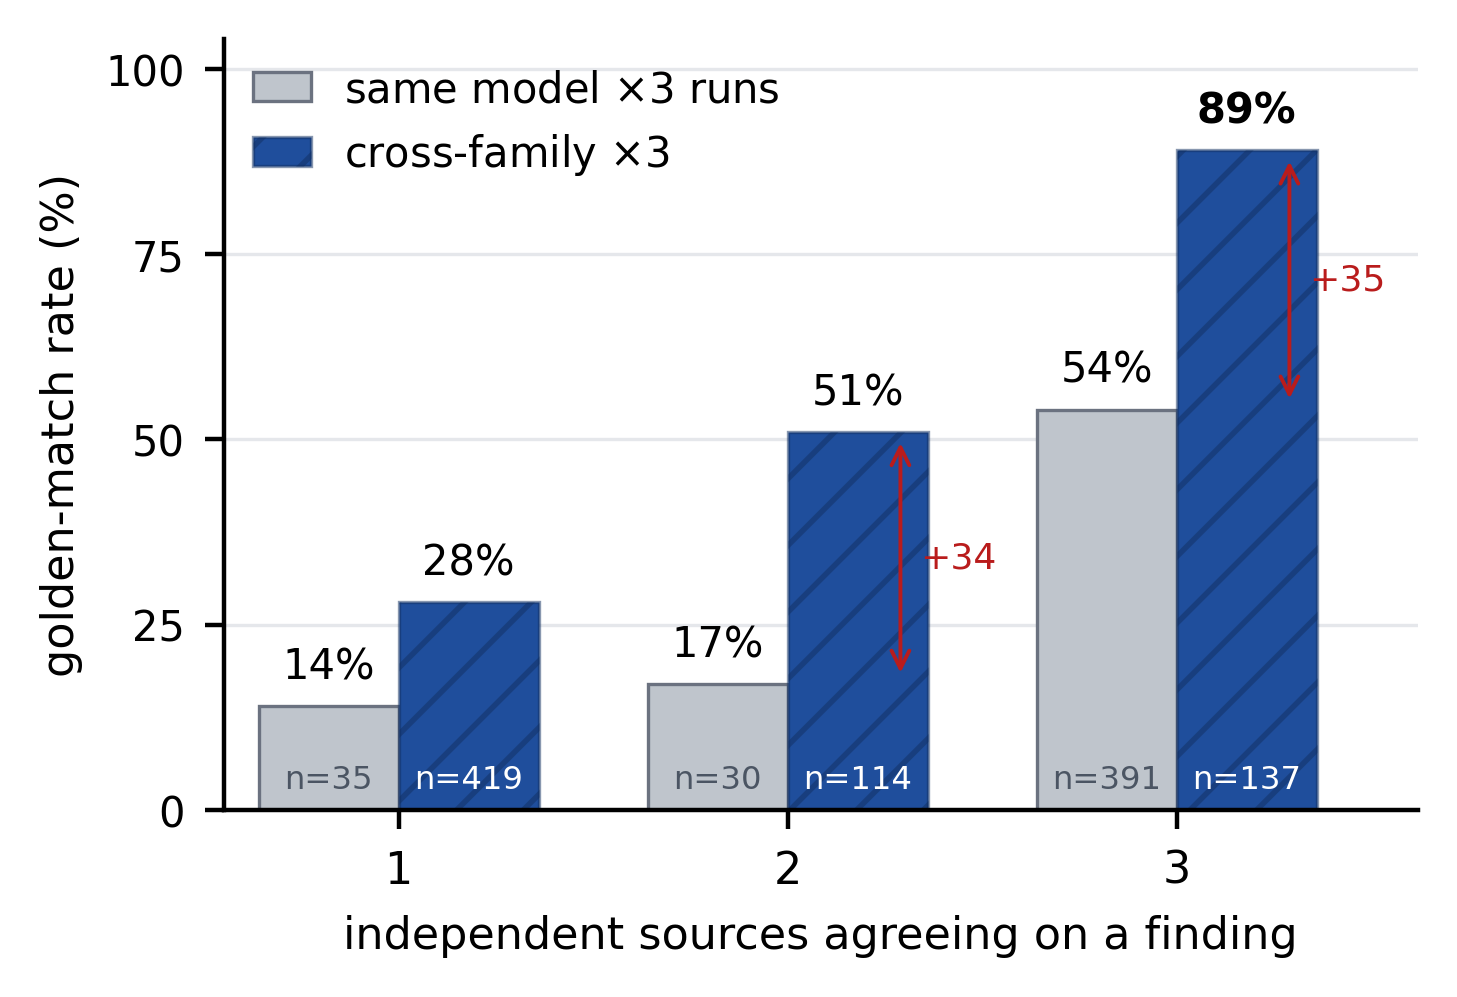
\includegraphics[width=\columnwidth]{fig2_depth_gradient.png}
\caption{Benchmark data only (injected-defect ground truth). Agreement predicts
truth only when the agreeing sources are
\emph{independent}. Repeating one model three times barely improves on a single
run until full recurrence, and saturates at that model's error ceiling (54\%);
three independent families reach 89\%. The gap at equal depth---${+}34$ and
${+}35$ points---is the correlated-error mechanism made visible. This benchmark
relationship reaches its ecological boundary on unlabeled industrial code, where
correctness labels are absent (Section~\ref{sec:industrial}).}
\label{fig:depth}
\end{figure}

\subsection{Where the signal lives: functional bugs, not conventions}
\label{sec:signal}
Cross-family agreement concentrates on one class of defect. On the 80-PR set
stratified by Qodo's two injected kinds (Fig.~\ref{fig:support}b), universal
\emph{functional} bugs are recovered far more often at every depth than
project-specific \emph{rule} violations. The ${\geq}2$-family set is 52\%
functional true positives, 20\% rule true positives, and 28\% golden-unmatched---
a high-precision filter for correctness defects, not a substitute for
project-specific linting.

\begin{figure*}[t]
\centering
% Generated by figures/make_figures.py (or figures/figures.ipynb).
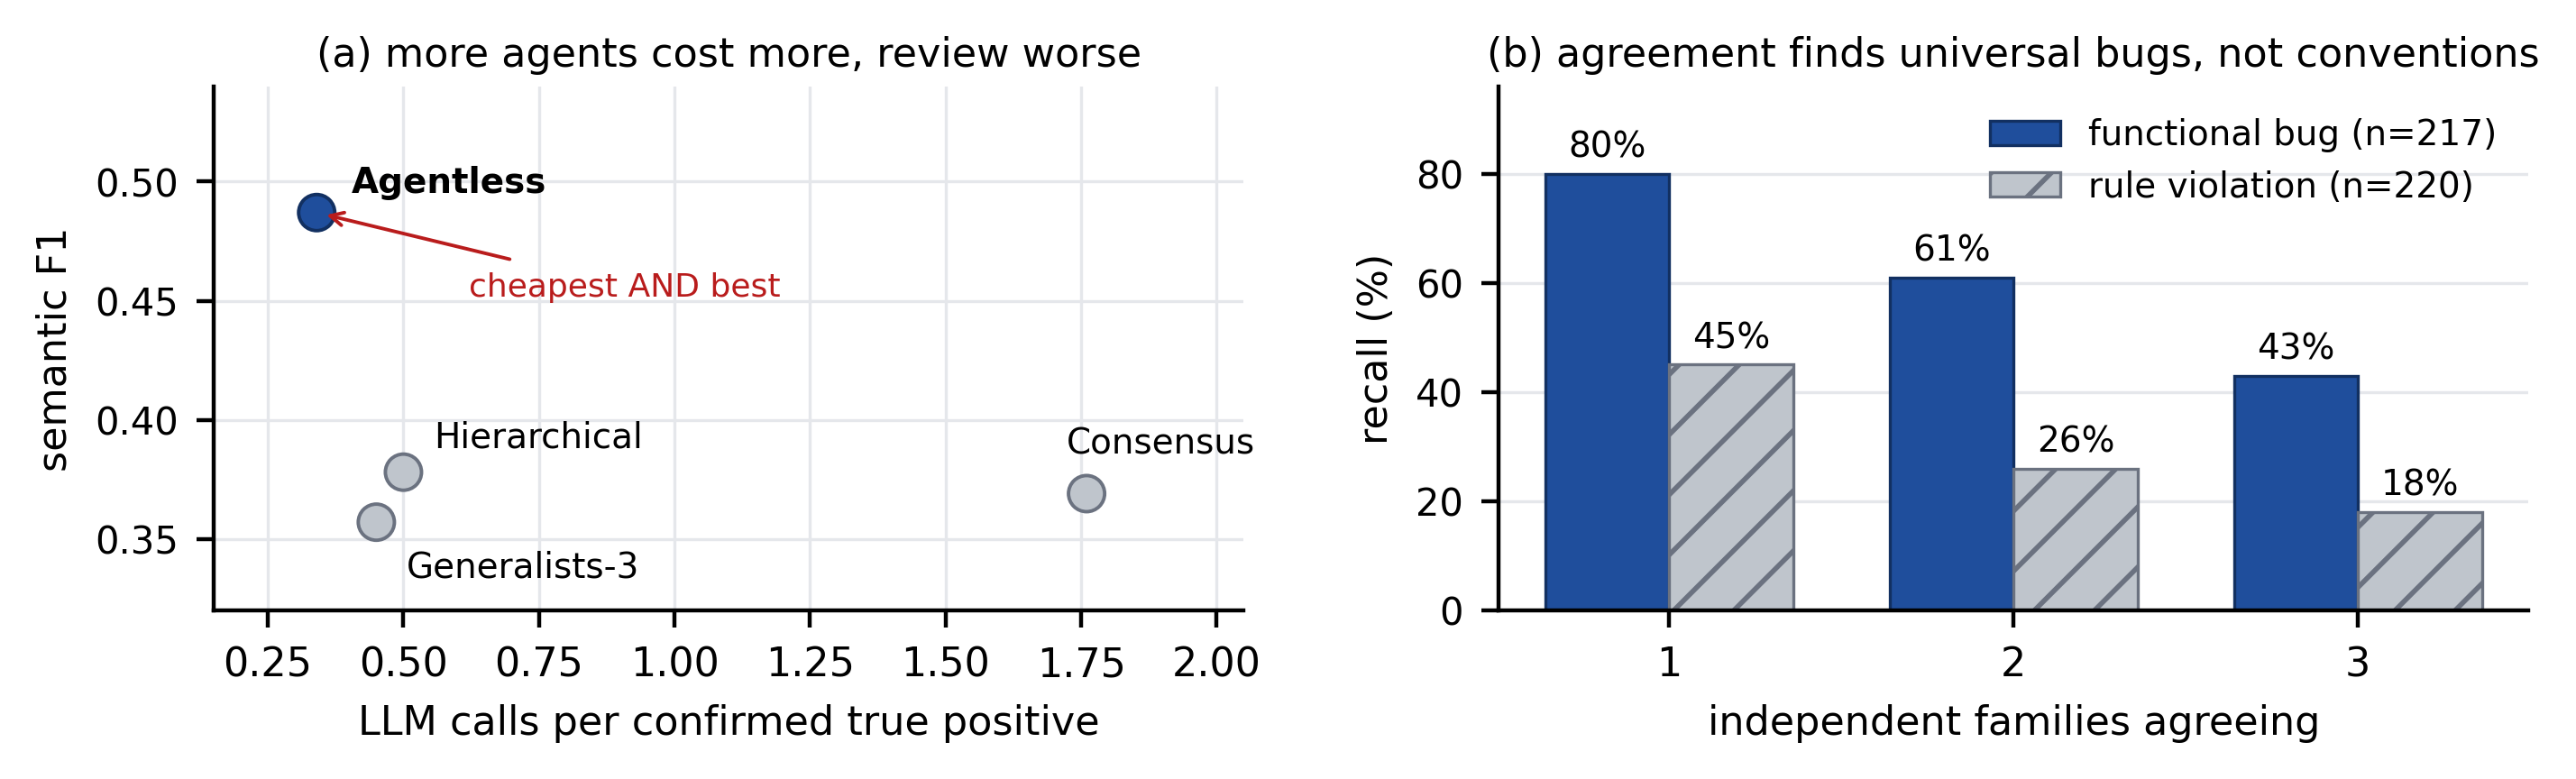
\includegraphics[width=\textwidth]{fig3_support.png}
\caption{\textbf{(a)} Accuracy/cost frontier: Agentless Pareto-dominates---
cheapest (0.34 LLM calls per confirmed true positive) and most accurate (semantic
F1 0.487), while Consensus costs $5\times$ more for a worse review.
\textbf{(b)} Cross-family agreement recovers universal functional bugs far more
often at every depth than project-specific rule violations, which a reviewer
without repository context cannot know.}
\label{fig:support}
\end{figure*}

\subsection{The recall axis: a decorrelation ladder with a ceiling (exploratory)}
\label{sec:ceiling}
Communication settled, we ask how far decorrelated \emph{sampling} alone can
reach, and what the residue requires. Unioning $K$ temperature or cross-family
draws saturates by ${\sim}4$ sources (Table~\ref{tab:ladder}), and the union of
\emph{all} eleven configurations we ran (seven model families, a conditioned
resampler, a temperature sweep) reaches only 0.83 recall (97 PRs), no single
source worth more than ${\sim}2$ points by leave-one-out---a robust ceiling.
(Nova~Pro is both a union member and the clustering judge here; this mild
circularity is confined to the exploratory union, not the confirmatory contrast
of Section~\ref{sec:hetero}.) The residue is structured: ${\sim}65\%$ are
repository conventions (36\% of rule violations are reached by \emph{no}
source---a \emph{correlated} blind spot) and ${\sim}15\%$ a repo-integrated
functional hard-core. A deterministic linter out-recalls the eleven-source union
on its target convention rules (0.54 vs.\ 0.46; hybrid 0.61), so the remaining
limitation is evidence, not model diversity---and no precision back-end
(agreement or aspect verification) lifts F1 above a plain union. The
saturation-to-a-ceiling phenomenon is not Qodo-specific: on 50 c-CRAB
PRs~\cite{crab} (real review comments---a different oracle), unioning the same
seven families lifts comment coverage from 36\% (Haiku alone) to a 55\% ceiling
that saturates by the second-to-third family---a different absolute value under a
different oracle, but the identical plateau.

\begin{table}[t]
\caption{Union recall by number of draws $K$ (semantic matching, 97 Qodo PRs).
Homo $=$ one model (Haiku) at $T{=}0.7$; hetero $=$ Haiku plus one distinct
family per rung (Kimi, GLM, DeepSeek, Nova, Llama~4, Palmyra).}
\label{tab:ladder}
\centering
\footnotesize
\begin{tabular}{@{}lccccccc@{}}
\toprule
$K$ & 1 & 2 & 3 & 4 & 5 & 6 & 7 \\
\midrule
Homo ($T{=}0.7$)  & 0.49 & 0.58 & 0.61 & --- & --- & --- & --- \\
Hetero (families) & 0.51 & 0.61 & 0.64 & 0.65 & 0.65 & 0.66 & 0.66 \\
\bottomrule
\end{tabular}
\\[2pt]{\footnotesize Diversity bonus (hetero $-$ homo) $=$ ${+}0.03$ at
$K{=}2,3$. Family order affects per-step marginals, not the $K{=}\max$ total.}
\end{table}

\subsection{Neither capability nor generation-side structure closes the gap}
\label{sec:nulls}
Three further generation-side interventions also fail to overcome the ceiling.
\emph{Capability (registered):} a stronger model does not target functional
bugs---on the 80-PR remainder the difference-in-differences is null
($\mathrm{DiD}{=}{-}1.8$, CI $[-8.6,5.5]$, $p{=}0.68$), Sonnet~4.5 lifting both
types over Haiku equally (functional $0.70{\to}0.74$, rule $0.32{\to}0.37$).
\emph{Module decomposition (exploratory):} per-module agents unioned beat one
whole-PR review by ${+}6.4$ recall ($p{=}0.016$), but only through the
${\sim}2.6\times$ compute---at a matched budget module-union \emph{trails} plain
multi-sampling (0.54 vs.\ 0.57, n.s.). \emph{Prompt specialization
(exploratory):} convention-only and functional-only personas suppress output
(5.3 vs.\ 16.1 findings/PR) and \emph{reduce} per-type recall (conventions 24\%
vs.\ 32\%, functional 59\% vs.\ 68\%), the team reaching recall 0.47, below the
generalist (0.50). Prompt personas are a \emph{negative} decorrelation source:
specialization pays only when it changes the detection \emph{mechanism}---a
checker, an independent family, or execution---not the prompt.

\subsection{Execution begins to reach what reading cannot (exploratory)}
\label{sec:execution}
The functional hard-core resists reading in every form we tried. Passive context
(whole changed files plus one-hop dependencies) does not raise recall over the
diff alone ($0.37{\to}0.35$, n.s., 50 PRs~\cite{crab}), and a read-only
repository-navigating agent (158 PRs) raises precision (0.17 vs.\ 0.13) at
\emph{lower} recall---agency verifies and prunes, not a coverage lever. Asked to
write self-contained reproductions for functional findings, a model succeeds on
only ${\sim}15\%$ ($n{=}20$), declining the rest as inseparable from repository
or runtime---the hard-core is genuinely repo-integrated. Real execution changes
this: on runtime-error SWE-bench instances whose issue text does not localize the
defect, feeding the reviewer the failing-test traceback lifts file-localization
recall from 1/6 to 5/6 (25\% to 100\% where the traceback names the fix file),
while on feature-addition instances it is a ceiling (both 100\%). Execution
recovers exactly the repo-integrated functional defects that diff reading and
read-only navigation cannot (small $n$, single model;
directional)~\cite{swereview}.

\subsection{How complete is the oracle?}
\label{sec:completeness}
Every precision figure above is measured against the injected golden set, so its
completeness bounds their interpretation. We audited it confirmatorily: three
independent judge families read every golden-\emph{unmatched} finding against the
diff (``does this identify a genuine problem?''), plus a calibration pass on
golden-\emph{matched} findings. Llama~3.3 calls 76\% of unmatched findings real
(92\% on known defects); Mistral Large~3 calls 73\% (90\%); DeepSeek~V3.2 calls
only 33\% (71\%).

The disagreement is definitional, not capability: DeepSeek is a strict
under-caller (rejecting ${\sim}29\%$ of \emph{known} defects) while the lenient
judges accept warranted concerns. Inter-judge agreement is poor
($\kappa{=}0.23$--$0.58$, and under prevalence-robust AC1/PABAK) against the
matcher's $\kappa{=}0.95$: whether two findings describe the same issue is
judge-stable, whereas whether a finding is a real bug is not settled by an LLM
judge of any size.

Three conclusions survive every definition: the golden set is materially
incomplete, so golden-referenced precision \emph{understates} all arms equally
(relative comparisons intact); the ${\geq}2$-family set's effective precision is
86--95\%; and false positives are less false than they appear (21--32\% are
localization near-misses, and high-severity findings are almost always real). The
magnitude awaits human adjudication; the direction does not---and removing the
golden set, as E3 does, leaves only the correctness signal that was already
unreliable.

\subsection{Industrial validation: the ecological boundary of cross-family
verification}
\label{sec:industrial}
E3 removes the oracle entirely: it asks whether the confirmed cross-family
verification signal (Section~\ref{sec:hetero}) survives when authoritative
correctness labels disappear---a boundary test for one relationship, not another
dataset comparison. On 30 real merged PRs (627 reviews: the four-arm ladder plus
the cross-family axis), scored with the same instruments but proxies for golden
labels, two patterns transfer: the communication-cost ladder is unchanged
(Agentless 1 call / 13\,s to Consensus 9 calls / 173\,s), and pool coverage gives
the same verdict---more agents do not buy coverage (single-pass highest at 0.27,
Consensus lowest at 0.10; pool coverage differs from golden recall, so we compare
directions, not ranks).

The cross-family verification signal, however, does not \emph{transfer} to this
setting: with no correctness labels the gradient of Fig.~\ref{fig:depth} cannot be
measured. Cross-family agreement is rare: only 23
findings reach depth-2 and 5 reach depth-3 of 904 clusters, versus 114 and 137 on
E1. More decisively, the genuineness judges disagree almost completely---Nova
labels 99\% of findings genuine, DeepSeek 68\%, at
$\kappa{=}0.03$---so the depth$\rightarrow$precision relation is set by judge
choice, not corroboration: flat at 100\% under Nova, and \emph{inverted} under
the discriminating judge, where findings families agree on score 0\% versus 15\%
for solo findings. This is precisely the boundary
Section~\ref{sec:completeness} anticipated, now with no golden set left to bound
it: the objective matcher still works, and the subjective correctness judge does
not. The result is therefore about the \emph{measurement apparatus}, not the
underlying benchmark relationship, which remains untested rather than
overturned---with mutually inconsistent oracles and depth counts of 23 and 5,
cross-family agreement can here be neither confirmed nor refuted.

\subsection{Complexity interaction: the effect does not grow with PR complexity}
\label{sec:rq3}
The registered complexity stratifier (PR type) was not persisted, so we proxy it
by the number of files an instance's defects span (\textbf{exploratory}). No
interaction survives on any contrast (all Holm $p{\ge}0.42$, $|\delta|{\le}0.12$):
complexity degrades every arm by a similar margin and the ordering is stable, so
no topology rescues complex PRs. The only directional hint runs \emph{against} the
registered prediction (Consensus$-$Hierarchical recall $0.000$ on simple vs.\
$-0.119$ on complex PRs, Holm $p{=}1.0$).

% =============================================================================
\section{Threats to Validity}
\label{sec:threats}

\begin{itemize}
  \item \textbf{Construct.} E3 is proxy-scored (no oracle), with sparse
  cross-family agreement (23/5 clusters at depth 2--3), genuineness judges that
  disagree ($\kappa{=}0.03$), and one partly AI-authored codebase---the
  conditions it exists to expose. Even the benchmark golden set is incomplete, so
  golden-referenced precision is a lower bound applying to every arm identically;
  the pair judge's human validation is pending.
  \item \textbf{Internal.} Model, prompts, evaluation pipeline, and a
  byte-identical snapshot are fixed while only sampling budget, roles, and
  communication vary; the compute-matched Generalists-3 control separates
  specialization from sampling, and evaluation replays deterministically.
  \item \textbf{External.} Qodo is synthetic-injection, so absolute scores sit on
  a favorable setting (within-benchmark comparisons hold); SWE-PRBench and E3
  partly offset this. The Sonnet~4.5 robustness arm has now completed at
  confirmatory scale ($N{=}99$) and replicates every registered conclusion
  (Section~\ref{sec:generation}), so model-robustness of the ranking is shown
  rather than assumed; the exploratory extensions are
  small-$n$, single-benchmark probes (execution directional, $n{=}6$). Headline
  claims are confirmatory (registered sizes, paired tests, CIs, Holm); finer
  stratifications, RQ3, and the ceiling/capability/execution extensions are
  exploratory, labeled throughout.
\end{itemize}

% =============================================================================
\section{Conclusion}

Under a pre-registered, frozen-model design, none of the tested multi-agent
workflows improved automated code review. Role specialization adds nothing over
compute-matched sampling (the primary null), no arm exceeds the single-pass
baseline's F1, extra agents buy recall at a 3--9$\times$ larger per-run call
budget, the self-consistency rescue our own pilot suggested does not replicate,
and the effect does not grow with PR complexity. The \emph{verification} axis is
where multi-agent value lives: agreement between independent model families is a
registered precision instrument that survives a change of pair
judge---findings all three families produce match injected ground truth 89\% of
the time versus 54\% for one model repeating itself---and the signal concentrates
on functional bugs.

That instrument has a precondition. On real unlabeled code it could not be
validated---LLM correctness judges disagree at $\kappa{=}0.03$ while the objective
matcher stays reliable at $\kappa{=}0.95$---so the industrial result bounds
\emph{oracle-based validation}, not cross-family agreement itself. The guidance is
therefore conditional: on benchmark-like tasks, do not add homogeneous agents for
quality, and treat cross-family agreement as a trust signal to calibrate against a
project's own oracle.

The broader lesson is that increasing communication among LLM agents yields
diminishing returns once generation saturates; the remaining gains come from
expanding what reviewers can \emph{observe}---repository context, executable
evidence, and deterministic analyses---rather than from more deliberation among
language models. Future work is a fixed-definition \emph{human} adjudication (the
oracle these judges could not provide) and scaling the execution probe to
confirmatory strength.

\begin{thebibliography}{16}

\bibitem{chatdev}
C.~Qian et al., ``ChatDev: Communicative agents for software development,''
in \emph{Proc. ACL}, 2024.

\bibitem{metagpt}
S.~Hong et al., ``MetaGPT: Meta programming for a multi-agent collaborative
framework,'' in \emph{Proc. ICLR}, 2024.

\bibitem{agentless}
C.~S. Xia, Y.~Deng, S.~Dunn, and L.~Zhang, ``Agentless: Demystifying
LLM-based software engineering agents,'' arXiv:2407.01489, 2024.

\bibitem{swebench}
C.~E. Jimenez et al., ``SWE-bench: Can language models resolve real-world
GitHub issues?'' in \emph{Proc. ICLR}, 2024.

\bibitem{survey}
X.~Zhang et al., ``LLM-based multi-agent systems for software engineering:
Literature review, vision and the road ahead,'' arXiv preprint, 2024.

\bibitem{whyfail}
Y.~Li et al., ``Why do multi-agent LLM systems fail?'' arXiv preprint, 2025.

\bibitem{llmjudge}
L.~Zheng et al., ``Judging LLM-as-a-judge with MT-Bench and Chatbot Arena,''
in \emph{Proc. NeurIPS}, 2023.

% --- new references (week-12); author lists verified against arXiv. ---
\bibitem{cobbe}
K.~Cobbe, V.~Kosaraju, M.~Bavarian, M.~Chen, H.~Jun, L.~Kaiser, M.~Plappert,
J.~Tworek, J.~Hilton, R.~Nakano, C.~Hesse, and J.~Schulman, ``Training
verifiers to solve math word problems,'' arXiv:2110.14168, 2021.

\bibitem{verga}
P.~Verga, S.~Hofst\"atter, S.~Althammer, Y.~Su, A.~Piktus, A.~Arkhangorodsky,
M.~Xu, N.~White, and P.~Lewis, ``Replacing judges with juries: Evaluating LLM
generations with a panel of diverse models,'' arXiv:2404.18796, 2024.

\bibitem{panickssery}
A.~Panickssery, S.~R. Bowman, and S.~Feng, ``LLM evaluators recognize and
favor their own generations,'' arXiv:2404.13076, 2024.

\bibitem{pappu}
A.~Pappu, B.~El, H.~Cao, C.~di~Nolfo, Y.~Sun, M.~Cao, and J.~Zou,
``Multi-agent teams hold experts back,'' in \emph{Proc. ICML}, 2026
(arXiv:2602.01011).

\bibitem{selfmoa}
W.~Li, Y.~Lin, M.~Xia, and C.~Jin, ``Rethinking mixture-of-agents: Is
mixing different large language models beneficial?'' arXiv:2502.00674,
2025.

\bibitem{zietsman}
C.~Zietsman, ``The specification as quality gate: Three hypotheses on
AI-assisted code review,'' arXiv:2603.25773, 2026.

\bibitem{sclar}
M.~Sclar, Y.~Choi, Y.~Tsvetkov, and A.~Suhr, ``Quantifying language models'
sensitivity to spurious features in prompt design,'' in \emph{Proc. ICLR},
2024 (arXiv:2310.11324).

% --- week-13 additions (execution / grounding probes). ---
\bibitem{crab}
Y.~Zhang et al., ``Code review agent benchmark,'' arXiv:2603.23448, 2026.

\bibitem{swereview}
R.~Wang et al., ``SWE-Review: Closing the loop on issue resolution with agentic
code review,'' arXiv:2607.06065, 2026.

\end{thebibliography}

\end{document}
